\documentclass[tikz,border=10pt]{standalone}
\usepackage{amsmath}
\begin{document}
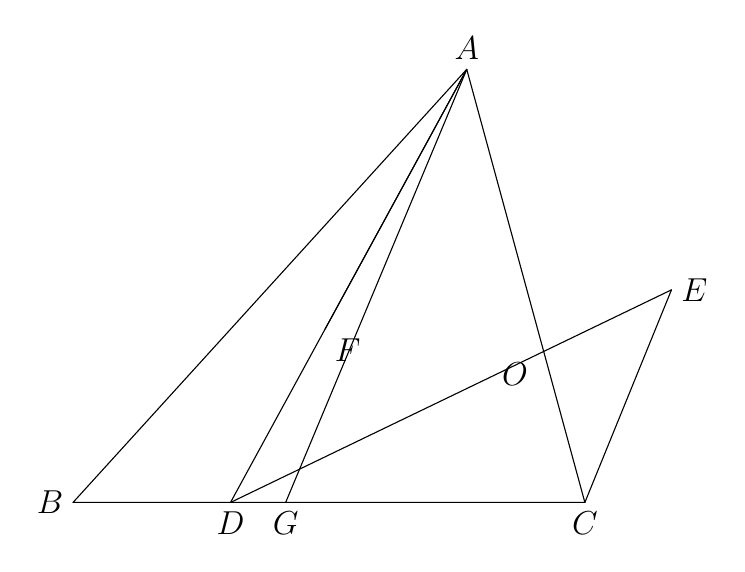
\begin{tikzpicture}[line cap=round, line join=round, font=\large]
\coordinate (A) at (5,5.5);
\coordinate (B) at (0,0);
\coordinate (C) at (6.5,0);
\coordinate (D) at (2,0);
\coordinate (G) at (2.7,0);
\coordinate (F) at (3.2,2.2);
\coordinate (E) at (7.6,2.7);
\coordinate (O) at (5.9,1.9);

\draw (A) -- (B) -- (C) -- cycle;
\draw (A) -- (D);
\draw (A) -- (G);
\draw (A) -- (F);
\draw (D) -- (E);
\draw (C) -- (E);
\draw (B) -- (C);

\node[above] at (A) {$A$};
\node[left] at (B) {$B$};
\node[below] at (C) {$C$};
\node[below] at (D) {$D$};
\node[below] at (G) {$G$};
\node[below right] at (F) {$F$};
\node[right] at (E) {$E$};
\node[below left] at (O) {$O$};
\end{tikzpicture}
\end{document}
